\documentclass[11pt]{article}
\usepackage[margin=1in]{geometry}
\usepackage[T1]{fontenc}
\usepackage{lmodern,amsmath,amssymb,booktabs,graphicx,xcolor,multirow,array}
\usepackage[numbers,sort&compress]{natbib}
\usepackage[colorlinks=true,linkcolor=blue,citecolor=blue,urlcolor=blue]{hyperref}
\newcommand{\todo}[1]{\textcolor{red}{\textbf{[TODO: #1]}}}
\newcommand{\pass}{\textsc{pass}}
\newcommand{\fail}{\textsc{fail}}

\title{How Much Data Do You Need to Validate a Trading Indicator?\\A Leakage-Safe, Power-Aware Protocol}
\author{Chintz Ruparel\\ Independent researcher}% EMAIL PLACEHOLDER: add contact email on this line before arXiv upload
\date{}
\begin{document}\sloppy
\maketitle
\begin{abstract}
New trading indicators are routinely declared useful on the strength of a single in-sample $t$-statistic, a shuffled cross-validation score or the best of many parameterisations. We specify and stress-test a simple protocol for deciding whether a candidate indicator adds out-of-sample predictive value over the historical mean: a point-in-time truncation audit, purged expanding walk-forward estimation with training-only standardisation, a Clark--West nested-model test on cross-sectionally averaged losses with Newey--West errors, and Holm control over the indicator family, all frozen in a pre-registered plan. In a synthetic panel with fat tails, volatility clustering and cross-sectional correlation (22{,}000 simulated studies) the protocol holds its nominal size (null rejection 1.6--5.6\% across 16 panel shapes, 500 replications each), whereas the common pooled OLS $t$-test on overlapping 5-day returns rejects a useless indicator 19--24\% of the time. Power is the binding constraint: an indicator with a daily information coefficient (IC) of 0.01 needs about 10 years of 50 tickers, or 20 years of 25, to be detected with 80\% probability; at IC~0.005 no panel in our grid reaches 60\%. A truncation audit flags three typical look-ahead constructions in 100\% of checks and six classic indicators in 0\%; one such leak (a centred moving average) yields an apparent out-of-sample $R^2$ of 0.41 on real ETF data. Applied to RSI, MACD, 12--1 momentum, one-month reversal, realised volatility and the 200-day moving-average gap on 38 liquid ETFs (development 2000--2019, one-shot holdout 2020--2026), no indicator adds predictive value at a 5- or 21-day horizon (all Holm $p=1.0$, all out-of-sample $R^2\le 0.0001$). A semi-synthetic check on the same real returns shows the panel had 83\% power for IC~0.01, so the null is informative: these indicators carry less than roughly that much linear predictive content for these assets.
\end{abstract}

\section{Introduction}
Technical analysis has a long and contested empirical record: early support for moving-average and breakout rules \citep{brock1992} weakens after data-snooping corrections \citep{sullivan1999}, and surveys report mixed results \citep{park2007}. In equity-premium prediction, \citet{welch2008} show that most predictors that look strong in sample fail out of sample, and \citet{campbell2008} propose the out-of-sample $R^2$ against the historical mean as the natural yardstick. Across hundreds of anomalies, many do not replicate \citep{hou2020}, consistent with high false-positive rates in research that searches many specifications \citep{harvey2015,bailey2014,ioannidis2005}.

Two failures are especially common when a practitioner evaluates a new indicator. The first is \emph{invalid inference}: overlapping multi-day returns combined with a persistent predictor make ordinary standard errors far too small \citep{hodrick1992,stambaugh1999}, and shuffled cross-validation leaks information across adjacent dates \citep{arlot2010,bergmeir2012}. The second is \emph{low power}: even a genuine indicator with a small IC is hard to distinguish from noise in a few tickers and a few years, so a ``failed'' test is often uninformative. Practitioners rarely know which situation they are in.

We contribute a compact, reusable protocol and quantify both failures:
\begin{enumerate}
\item A leakage-safe evaluation protocol for any candidate indicator (\S\ref{sec:protocol}), with a pre-registered analysis plan frozen (and hashed) before any synthetic grid or real run.
\item A size and power study over 22{,}000 synthetic studies (\S\ref{sec:power}), giving the history needed to detect a given IC, and showing that the protocol holds size while a common shortcut does not.
\item Four leakage demonstrations (\S\ref{sec:leak}): overlapping-label inference, look-ahead indicators caught by a truncation audit, shuffled cross-validation, and specification search.
\item An application to six classic indicators on 38 free-data ETFs with a one-shot holdout (\S\ref{sec:real}), interpreted through the power study so that a null result carries information.
\end{enumerate}
We make no profitability claims and do not model trading costs; the question is only whether the indicator improves forecasts.

\section{Related Work}
\paragraph{Out-of-sample evaluation of predictors.} \citet{diebold1995} test equal predictive accuracy; for nested models the Diebold--Mariano statistic is undersized, which \citet{clark2007} correct with an adjusted mean-squared-prediction-error (MSPE) difference. \citet{welch2008} and \citet{campbell2008} established out-of-sample $R^2$ relative to the historical mean as the benchmark for return predictors. We use Newey--West standard errors \citep{newey1987}; stationary-bootstrap alternatives exist \citep{politis1994}.
\paragraph{Overlapping returns and persistent predictors.} \citet{hodrick1992} documents the size distortions from overlapping long-horizon returns, and \citet{stambaugh1999} the small-sample bias of predictive regressions with persistent regressors.
\paragraph{Data snooping and multiple testing.} The Reality Check \citep{white2000}, the SPA test \citep{hansen2005} and stepwise procedures \citep{romano2005} control snooping across models; Holm's step-down \citep{holm1979} and false-discovery control \citep{benjamini1995} handle families of tests. \citet{bailey2014,bailey2016} and \citet{bailey2014b} quantify backtest overfitting and deflate Sharpe ratios, and \citet{harvey2015,harvey2015b} argue for higher hurdles.
\paragraph{Leakage.} \citet{kaufman2012} formalise leakage in data mining and its detection. Cross-validation for dependent data is reviewed by \citet{arlot2010} and \citet{bergmeir2012}.
\paragraph{The indicators.} Momentum is documented cross-sectionally \citep{jegadeesh1993} and in time series \citep{moskowitz2012}; moving-average rules are studied by \citet{brock1992}, and pattern-based technical analysis by \citet{lo2000}.
Our contribution is not a new test statistic: it is a packaged protocol plus an explicit size/power map in panel shape, which tells a practitioner in advance whether their data can answer the question.

\section{Protocol}\label{sec:protocol}
Let $r_{i,t}$ be the daily log return of asset $i$ and $x_{i,t}$ the candidate indicator, computed from data up to the close of $t$. The target is the $h$-day forward return $y_{i,t}=\sum_{k=1}^{h} r_{i,t+k}$, with $h=5$ (primary) and $h=21$ (secondary).
\begin{enumerate}
\item \textbf{Point-in-time audit.} For 25 random dates $t$ we recompute the indicator on the series truncated at $t$ and compare with the value from the full series. Any mismatch flags look-ahead.
\item \textbf{Purged walk-forward.} Test blocks of 126 dates follow an initial 252 dates; each block's training set is all earlier dates whose label window ends before the block starts (a purge of $h$ dates). Indicators are winsorised at the 1st/99th percentiles and standardised with training statistics only.
\item \textbf{Nested forecasts.} Benchmark: the training mean of $y$. Augmented: pooled OLS $y=\alpha+\beta z+\varepsilon$ on the standardised indicator $z$.
\item \textbf{Test.} For each test date we average across available assets the Clark--West term $f_{i,t}=e_{b,i,t}^2-\left(e_{a,i,t}^2-(\hat y_{b,i,t}-\hat y_{a,i,t})^2\right)$. Averaging per date absorbs cross-sectional correlation. We test $\mathbb E f>0$ one-sided with a Newey--West standard error, lag $\max(h,\lceil 4(n/100)^{2/9}\rceil)$. We also report the Diebold--Mariano $t$ and out-of-sample $R^2=1-\mathrm{SSE}_a/\mathrm{SSE}_b$.
\item \textbf{Family control.} Holm adjustment across the pre-registered indicator family.
\end{enumerate}
The analysis plan (grids, seeds, universe, indicators, dates) was written and SHA-256 hashed before any run (\texttt{code/results\_ivp/ANALYSIS\_PLAN.md}). One amendment followed: an optional \texttt{score\_from} argument restricts scoring to holdout dates, with the default leaving earlier results unchanged.

\section{Size and Power}\label{sec:power}
\paragraph{Data-generating process.} The indicator follows an independent AR(1) per asset ($\phi=0.95$, unit variance). Returns are $r_{i,t+1}=b\,x_{i,t}+\sigma_{i,t+1}\epsilon_{i,t+1}$ with $\epsilon=\sqrt{\rho}f_t+\sqrt{1-\rho}u_{i,t}$, standardised $t_5$ shocks, GARCH(1,1) volatility $(0.02,0.08,0.90)$, and $b$ set so that $\operatorname{corr}(x_t,r_{t+1})=$ IC. The grid covers IC $\in\{0,0.0025,0.005,0.01,0.02\}$, $N\in\{5,10,25,50\}$ and $\{3,5,10,20\}$ years at $\rho=0.3$, with 500 seeds per null cell and 200 per non-null cell. A sensitivity check varies $\rho\in\{0,0.6\}$.

\paragraph{Size.} Table~\ref{tab:size} shows that the protocol's null rejection rate stays between 1.6\% and 5.6\%. Every cell's 95\% Wilson interval contains 5\% or lies below it, and the test becomes conservative at 20 years. The Diebold--Mariano statistic is badly undersized for these nested models (0--1.4\%), as \citet{clark2007} predict. The naive pooled OLS $t$-test on the same data rejects 19--24\% of the time.

\begin{table}[h]\centering\small
\caption{Rejection rate under the null (IC $=0$, $\rho=0.3$, 500 seeds per cell, one-sided 5\%).}\label{tab:size}
\begin{tabular}{l rrrr rrrr}\toprule
& \multicolumn{4}{c}{Protocol (Clark--West, HAC)} & \multicolumn{4}{c}{Naive pooled OLS $t$}\\ \cmidrule(lr){2-5}\cmidrule(lr){6-9}
$N$ \textbackslash{} years & 3&5&10&20 & 3&5&10&20\\\midrule
5  & .042&.050&.044&.022 & .192&.206&.220&.226\\
10 & .056&.044&.054&.036 & .208&.222&.220&.234\\
25 & .044&.042&.044&.016 & .240&.228&.234&.194\\
50 & .032&.048&.036&.016 & .198&.222&.216&.232\\\bottomrule
\end{tabular}\end{table}

\paragraph{Power.} Figure~\ref{fig:power} and Table~\ref{tab:power} show the results. With 5 tickers no cell reaches 80\% power below IC $=0.02$, and even IC $=0.02$ reaches only 73\% at 20 years. At IC $=0.01$, 80\% power needs 50 tickers for 10 years (0.84) or 25 tickers for 20 years (0.82). At IC $\le 0.005$ the best cell is 0.58 (50 tickers, 20 years). Cross-sectional correlation matters less than expected in this range: at $N=25$, 10 years and IC $=0.01$, power is 0.64, 0.55 and 0.63 for $\rho=0,0.3,0.6$.

\begin{figure}[h]\centering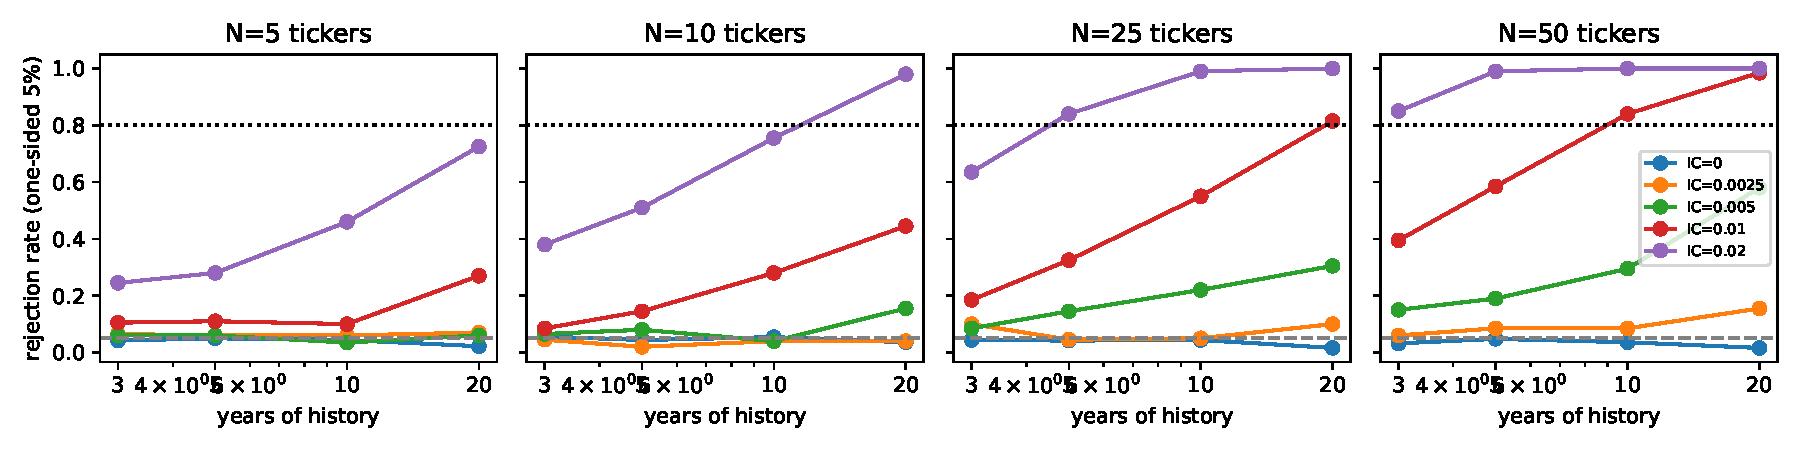
\includegraphics[width=\linewidth]{fig_ivp_power.pdf}
\caption{Rejection rate of the protocol by panel shape and IC (200 seeds per non-null cell, 500 null). Dotted: 80\%; dashed: 5\%.}\label{fig:power}\end{figure}

\begin{table}[h]\centering\small
\caption{Power at one-sided 5\% ($\rho=0.3$, 200 seeds). Bold: $\ge 0.80$.}\label{tab:power}
\begin{tabular}{ll rrrr}\toprule
IC & $N$ & 3y & 5y & 10y & 20y\\\midrule
0.005 & 25 & .085 & .145 & .220 & .305\\
0.005 & 50 & .150 & .190 & .295 & .580\\
0.01 & 10 & .085 & .145 & .280 & .445\\
0.01 & 25 & .185 & .325 & .550 & \textbf{.815}\\
0.01 & 50 & .395 & .585 & \textbf{.840} & \textbf{.985}\\
0.02 & 5 & .245 & .280 & .460 & .725\\
0.02 & 10 & .380 & .510 & .755 & \textbf{.980}\\
0.02 & 25 & .635 & \textbf{.840} & \textbf{.990} & \textbf{1.00}\\
0.02 & 50 & \textbf{.850} & \textbf{.990} & \textbf{1.00} & \textbf{1.00}\\\bottomrule
\end{tabular}\end{table}

\section{Leakage Demonstrations}\label{sec:leak}
\begin{description}
\item[L1, overlapping labels.] Null DGP, 10 tickers, 5 years, 200 seeds. The naive pooled $t$-test rejects 22.0\% (95\% CI 16.8--28.2\%); the protocol rejects 4.0\% (2.0--7.7\%).
\item[L2, look-ahead indicators.] Three leaky constructions are a centred 21-day moving-average gap, a z-score using full-sample mean and standard deviation, and a feature built from the next day's return. The truncation audit on SPY flags each in 25/25 checks and each of the six classic indicators in 0/25. Without the audit, the walk-forward test is fooled on real ETF development data: the centred-MA leak gives $t_{CW}=19.2$ and out-of-sample $R^2=0.41$, and the next-day leak gives $t_{CW}=6.9$ and $R^2=0.025$. The full-sample z-score gives only $t=1.67$ ($p=0.047$), because its leak is mild. Walk-forward splitting therefore does not catch feature-level leakage; the audit is a necessary separate step.
\item[L3, shuffled $k$-fold.] We fit a $k$NN regressor ($k=50$) on $[x,\,$20-day lagged return$]$ under the null, 100 seeds. The shuffled 5-fold out-of-sample $R^2$ is positive in 6\% of seeds (median $-0.012$), versus 1\% for purged walk-forward (median $-0.023$). The inflation is real but modest in this configuration; we report it as weak evidence and do not generalise it to more flexible learners.
\item[L4, specification search.] We pick the best of 20 momentum lookbacks (5--300 days) by minimum $p$, under the null with 200 seeds. The unadjusted best-of-20 rejects 41.5\% (34.9--48.4\%). Holm brings this to 8.0\% (5.0--12.6\%), which is still above nominal. With persistent, return-based regressors, the per-test asymptotic size is slightly liberal in this short (5-year, 10-ticker) panel, and Holm does not fully repair that.
\end{description}

\section{Application to Classic Indicators}\label{sec:real}
\paragraph{Data.} We use the 38-ETF universe frozen for a companion study before any download: US size and style funds, sectors, country funds, rates and credit, real estate, and commodities. Data are Yahoo adjusted closes from 2000 to 2026-10-19, an unbalanced panel in which the last fund starts in April 2007, with mean pairwise daily correlation 0.40. Indicators are RSI(14), the MACD(12,26,9) histogram divided by price, 12--1 month momentum, one-month reversal, 21-day realised volatility, and the log gap to the 200-day moving average. All six pass the truncation audit. The development period is 2000--2019, and the holdout (2020-01-01 onward) was unlocked once, after the development results were written.

\begin{table}[h]\centering\small
\caption{Clark--West $t$ (one-sided), Holm-adjusted $p$ and out-of-sample $R^2$ (\%) per indicator. Dev: 4{,}774 test dates ($\approx$169k obs); holdout: 1{,}704 dates (64{,}752 obs).}\label{tab:real}
\begin{tabular}{l rrr rrr}\toprule
& \multicolumn{3}{c}{Dev, $h=5$} & \multicolumn{3}{c}{Holdout, $h=5$}\\\cmidrule(lr){2-4}\cmidrule(lr){5-7}
Indicator & $t_{CW}$ & $p_{Holm}$ & $R^2_{oos}$ & $t_{CW}$ & $p_{Holm}$ & $R^2_{oos}$\\\midrule
RSI14 & $-0.01$ & 1.0 & $-0.11$ & $0.04$ & 1.0 & $-0.02$\\
MACD hist. & $0.36$ & 1.0 & $-0.07$ & $-0.84$ & 1.0 & $-0.33$\\
MOM 12--1 & $-0.71$ & 1.0 & $-0.19$ & $-1.69$ & 1.0 & $-0.02$\\
REV 1M & $-0.11$ & 1.0 & $-0.16$ & $-0.24$ & 1.0 & $-0.05$\\
RVOL21 & $-1.40$ & 1.0 & $-0.45$ & $-0.43$ & 1.0 & $-0.06$\\
MA200 gap & $-0.73$ & 1.0 & $-0.25$ & $-0.59$ & 1.0 & $-0.04$\\\bottomrule
\end{tabular}\end{table}

At $h=21$, every Holm $p$ is 1.0 in both periods. The largest holdout out-of-sample $R^2$ is $+0.01\%$ (RSI14), with $t_{CW}=0.36$.

\paragraph{Is this null informative?} We inject a synthetic AR(1) indicator of known IC into the \emph{real} development-period returns and rerun the protocol, 100 seeds per level. This check was exploratory and not pre-registered. Rejection rates are 1\% at IC $=0$, 33\% at 0.005, 83\% at 0.01 and 100\% at 0.02, in line with the synthetic grid for a panel of this size. The development-period null therefore excludes, with about 80\% power, a linear daily IC near 0.01 or larger for these indicators on these assets. It says nothing about nonlinear use, other assets, intraday data or trading rules with position sizing.

\section{Discussion and Limitations}
\textbf{Practical rule.} Before testing an indicator, read the power table: with five tickers and a few years, a test of a realistic IC (0.005--0.01) is close to a coin flip with a 5\% chance of heads, and a failure to reject means little. \textbf{Limitations.} (i) The DGP is linear with an independent AR(1) indicator; indicators that are themselves functions of past returns, as in L4, are slightly liberal in short panels. (ii) We test linear pooled forecasts only; nonlinear models need their own power analysis. (iii) Yahoo data are free but licensed for personal use; a licensed re-run would strengthen the application. (iv) There are no transaction costs or economic-value measures. (v) The kNN demonstration (L3) is weak; we report it as such. (vi) The six indicators use standard parameter choices; we did not search them, by design.

\section{Conclusion}
A leakage-safe, nested, cross-sectionally aggregated walk-forward test holds its size where the common shortcut rejects a useless indicator about one time in five. Detecting a realistic daily IC of 0.01 needs on the order of 250--500 ticker-years. Six classic indicators show no out-of-sample value on 38 ETFs, and the power analysis shows that this null is informative.

\paragraph{Code and data availability.} Code: \url{https://github.com/ChintzRuparel/indicator-validation-protocol}. All synthetic results regenerate from \texttt{code/run\_power.py}, \texttt{run\_leakage.py}, \texttt{run\_real.py} and \texttt{run\_real\_extra.py}.
\paragraph{Data statement.} Daily ETF prices are from Yahoo Finance (via \texttt{yfinance}), which provides them for personal use only. The prices are not redistributed: the repository contains only code, the frozen symbol list and SHA-256 hashes of the input files, and users re-download the data with the released script.
\paragraph{Author disclosure.} This work was done independently, outside the author's employment, and uses no employer data, code or resources. It received no funding. The author declares no competing interests. Nothing in this paper is investment advice.

\bibliographystyle{plainnat}
\bibliography{references}
\end{document}
